\renewcommand{\thesection}{\Roman{section}}
\titleformat{\section}
{\normalfont\bfseries}{PHẦN~\thesection.}{0.4em}{}
\newcolumntype{C}[1]{>{\centering\arraybackslash}p{#1}}
\newcolumntype{L}[1]{>{\raggedright\arraybackslash}p{#1}}
\begin{tabular}{C{5cm}C{11cm}}
	\textbf{TRUNG TÂM MANABIE}& \textbf{ĐỀ ÔN TẬP KIỂM TRA GIỮA HỌC KÌ 2} \\
	\textbf{ĐỀ 01}& \textbf{Môn: VẬT LÝ}\\
	\textit{(Đề có 05 trang)}& \textit{Thời gian làm bài: 50 phút, không kể thời gian phát đề}
	
	\noindent\rule{4cm}{0.8pt} \\
\end{tabular}
\hdc{
\section{}
Mỗi câu trả lời đúng thí sinh được \textbf{0,25 điểm}.
\begin{center}
	\begin{tabular}{|C{2.5cm}|C{4.0cm}|C{2.5cm}|C{4.0cm}|}
		\hline
		\thead{Câu} & \thead{Đáp án} & \thead{Câu} & \thead{Đáp án}\\
		\hline
		1 & B &  10 & A \\ 
		\hline
		2 & D &  11 & A \\ 
		\hline
		3 & C &  12 & A \\ 
		\hline
		4 & A &  13 & D \\ 
		\hline
		5 & B &  14 & A \\ 
		\hline
		6 & C &  15 & B \\ 
		\hline
		7 & C &  16 & C \\ 
		\hline
		8 & C &  17 & B \\ 
		\hline
		9 & B &  18 & C \\ 
		\hline
	\end{tabular}
\end{center}
\section{}
Điểm tối đa của 01 câu hỏi là \textbf{1 điểm}.
\begin{itemize}
	\item Thí sinh lựa chọn chính xác 01 ý trong 1 câu hỏi được \textbf{0,1} điểm.
	\item Thí sinh lựa chọn chính xác 02 ý trong 1 câu hỏi được \textbf{0,25} điểm.
	\item Thí sinh lựa chọn chính xác 03 ý trong 1 câu hỏi được \textbf{0,50} điểm.
	\item Thí sinh lựa chọn chính xác cả 04 ý trong 1 câu hỏi được \textbf{1} điểm.
\end{itemize}
\begin{center}
	\begin{tabular}{|C{1.0cm}|C{2.0cm}|C{3.0cm}|C{1.0cm}|C{2.0cm}|C{3.0cm}|}
		\hline
		\thead{Câu} & \thead{Lệnh hỏi} &\thead{Đáp án\\ (Đ/S)} &\thead{Câu} & \thead{Lệnh hỏi} &\thead{Đáp án\\ (Đ/S)}\\
		\hline
		\multirow{4}{*}{\textbf{1}}& a) & S & \multirow{4}{*}{\textbf{3}} & a) & Đ \\
		\cline{2-3}\cline{5-6}
									& b) & Đ &                             & b) & S \\
		\cline{2-3}\cline{5-6}
									& c) & Đ &                             & c) & S \\
		\cline{2-3}\cline{5-6}
									& d) & Đ &                             & d) & Đ \\
		\hline
		\multirow{4}{*}{\textbf{2}}& a) & S & \multirow{4}{*}{\textbf{4}} & a) & S \\
		\cline{2-3}\cline{5-6}
									& b) & Đ &                             & b) & Đ \\
		\cline{2-3}\cline{5-6}
									& c) & S &                             & c) & S \\
		\cline{2-3}\cline{5-6}
									& d) & S &                             & d) & Đ \\
		\hline		                           		                       
	\end{tabular}
\end{center}
\section{}
Mỗi câu trả lời đúng thí sinh được \textbf{0,25 điểm}.
\begin{center}
	\begin{tabular}{|C{2.5cm}|C{4.0cm}|C{2.5cm}|C{4.0cm}|}
		\hline
		\thead{Câu} & \thead{Đáp án} & \thead{Câu} & \thead{Đáp án}\\
		\hline
		1 & -15 &  4 & 8,17 \\ 
		\hline
		2 & X, Z, Y &  5 & 45 \\ 
		\hline
		3 & 9 &  6 & 6300 \\ 
		\hline
	\end{tabular}
\end{center}
\newpage
}

\setcounter{section}{0}
\section{Câu trắc nghiệm nhiều phương án lựa chọn.}
\textit{Thí sinh trả lời từ câu 1 đến câu 18. Mỗi câu hỏi thí sinh chọn một phương án.}
	\begin{enumerate}[label=\bfseries Câu \arabic*:]
		\item Cọ xát thanh ebonit vào miếng dạ, thanh ebonit tích điện âm vì
		\begin{mcq}
			\item Electron chuyển từ thanh ebonit sang dạ.
			\item Electron chuyển từ dạ sang thanh ebonit.
			\item Proton chuyển từ dạ sang thanh ebonit.
			\item Proton chuyển từ thanh ebonit sang dạ.
		\end{mcq}
	\hideall{
\textbf{Đáp án B.}	
}
	
		
		\item Đặt hai điện tích $q_1$ và $q_2$ gần nhau thì thấy chúng hút nhau. Khẳng định nào sau đây là đúng?
		\begin{mcq}(2)
			\item $q_1$ và $q_2$ nhiễm điện dương.
			\item $q_1$ và $q_2$ cùng nhiễm điện âm.
			\item $q_1$ nhiễm điện dương, $q_2$ nhiễm điện âm.
			\item $q_1$ và $q_2$ nhiễm điện trái dấu.
		\end{mcq}
	\hideall{
\textbf{Đáp án D.}\\
Hai điện tích hút nhau khi đặt gần nhau $\Rightarrow$ hai điện tích trái dấu nhau.	
}

\item Cường độ điện trường tại một điểm đặc trưng cho
\begin{mcq}
	\item thể tích vùng có điện trường lớn hay nhỏ.
	\item điện trường tại điểm đó về phương diện dự trữ năng lượng.
	\item tác dụng lực của điện trường lên điện tích đặt tại điểm đó.
	\item tốc độ dịch chuyển của điện tích tại điểm đó.
\end{mcq}
\hideall{
\textbf{Đáp án C.}\\
Cường độ điện trường tại một điểm đặc trưng cho tác dụng lực của điện trường tại điểm đó.
}

\item Thế năng tĩnh điện của điện tích $q$ trong điện trường đặc trưng cho
\begin{mcq}
	\item khả năng sinh công của điện trường tại điểm đặt của $q$.
	\item khả năng tác dụng lực của điện trường tại điểm đặt của $q$.
	\item tác dụng mạnh hay yếu của điện trường tại điểm đặt của $q$.
\end{mcq}
\hideall{
\textbf{Đáp án A.}\\
Thế năng tĩnh điện của điện tích $q$ trong điện trường đặc trưng cho khả năng sinh công của điện trường tại điểm đặt của $q$.
}

\item Tụ điện là hệ gồm hai vật dẫn đặt
\begin{mcq}
	\item gần nhau và ngăn cách nhau bằng một lớp dẫn điện.
	\item gần nhau và ngăn cách nhau bằng một lớp cách điện.
	\item tiếp xúc với nhau và được bao bọc bằng điện môi.
	\item cách nhau một khoảng đủ xa.
\end{mcq}
\hideall{
\textbf{Đáp án B.}
}

\item Một tụ điện có điện dung $C$ được nạp điện với hiệu điện thế $U$. Tăng hiệu điện thế hai bản tụ lên gấp đôi (tụ vẫn chưa bị đánh thủng) thì điện tích của tụ
\begin{mcq}(4)
	\item không thay đổi.
	\item giảm 2 lần.
	\item tăng 2 lần.
	\item tăng 4 lần.
\end{mcq}
\hideall{
\textbf{Đáp án C.}\\
$$Q=CU$$
Khi $U$ tăng 2 lần thì điện tích của tụ cũng tăng 2 lần.
}

\item Đơn vị đo thế năng điện là
\begin{mcq}(4)
	\item watt $\left(\si{\watt}\right)$.
	\item volt $\left(\si{\volt}\right)$.
	\item joule $\left(\si{\joule}\right)$.
	\item coulomb $\left(\si{\coulomb}\right)$.
\end{mcq}
\hideall{
\textbf{Đáp án C.}
}

\item Đơn vị nào sau đây dùng để đo điện tích?
\begin{mcq}(4)
	\item volt $\left(\si{\volt}\right)$.
	\item newton $\left(\si{\newton}\right)$.
	\item coulomb $\left(\si{\coulomb}\right)$.
	\item ohm $\left(\si{\ohm}\right)$.
\end{mcq}
\hideall{
\textbf{Đáp án C.}\\
Đơn vị dùng để đo điện tích là coulomb $\left(\si{\coulomb}\right)$.
}

\item Đơn vị đo điện thế là volt $\si{\volt}$ với $\SI{1}{\volt}$ tương ứng là
\begin{mcq}(4)
	\item $\SI{1}{\joule\cdot\coulomb}$.
	\item $\SI{1}{\joule/\coulomb}$.
	\item $\SI{1}{\newton/\coulomb}$.
	\item $\SI{1}{\joule/\newton}$.
\end{mcq}
\hideall{
	\textbf{Đáp án B.}
}


\item Một điện tích $\SI{-1}{\micro\coulomb}$ đặt trong chân không sinh ra điện trường tại một điểm cách nó $\SI{1}{\meter}$ có độ lớn và hướng là
\begin{mcq}(2)
	\item $\SI{9000}{\volt/\meter}$, hướng về phía điện tích.
	\item $\SI{9000}{\volt/\meter}$, hướng ra xa điện tích.
	\item $\SI{9E9}{\volt/\meter}$, hướng về phía điện tích.
	\item $\SI{9E9}{\volt/\meter}$, hướng ra xa điện tích.
\end{mcq}
\hideall{
\textbf{Đáp án A.}\\
Độ lớn cường độ điện trường do điện tích gây ra:
$$E=\dfrac{k\left|q\right|}{\varepsilon r^2}=\SI{9000}{\volt/\meter}.$$
}

\item Hai tấm kim loại phẳng, nhiễm điện trái dấu, đặt song song cách nhau $\SI{2}{\centi\meter}$. Hiệu điện thế giữa hai tấm kim loại là $\SI{100}{\volt}$. Cường độ điện trường trong khoảng không gian giữa hai tấm là
\begin{mcq}(4)
	\item $\SI{5000}{\volt/\meter}.$
	\item $\SI{50}{\volt/\meter}$.
	\item $\SI{200}{\volt/\meter}$.
	\item $\SI{20}{\volt/\meter}$.
\end{mcq}
\hideall{
\textbf{Đáp án A.}\\
Cường độ điện trường trong khoảng không gian giữa hai tấm là
$$E=\dfrac{U}{d}=\SI{5000}{\volt/\meter}.$$
}

\item Hai quả cầu nhỏ có cùng điện tích $\SI{5E-6}{\coulomb}$ đặt cách nhau $\SI{30}{\centi\meter}$ trong không khí. Độ lớn lực tương tác giữa chúng là
\begin{mcq}(4)
	\item $\SI{2.5}{\newton}$.
	\item $\SI{2.5E-4}{\newton}$.
	\item $\SI{7.5E-3}{\newton}$.
	\item $\SI{0.75}{\newton}$.
\end{mcq}
\hideall{
\textbf{Đáp án A.}\\
Độ lớn lực tương tác giữa hai điện tích điểm:
$$F=\dfrac{k\left|q_1q_2\right|}{r^2}=\SI{2.5}{\newton}.$$
}

\item Hình vẽ nào sau đây mô tả đường sức của điện trường đều?
\begin{center}
	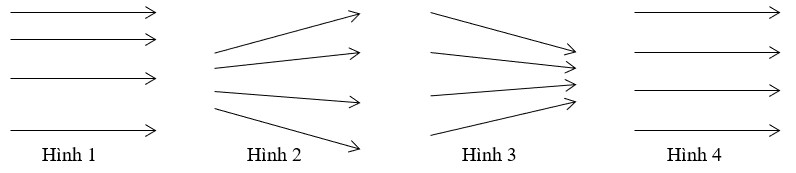
\includegraphics[width=0.8\linewidth]{../figs/PH11-MidSem2-01-1}
\end{center}
\begin{mcq}(4)
	\item Hình 1.
	\item Hình 2.
	\item Hình 3.
	\item Hình 4.
\end{mcq}
\hideall{
\textbf{Đáp án D.}
}

\item Hình bên mô phỏng đường sức điện của hai vật dẫn tích điện trái dấu và được đặt gần nhau. Bốn điểm W, X, Y và Z được đánh dấu trên hình vẽ. Đặt một điện tích khác ở vị trí nào trong 4 vị trí trên thì lực tĩnh điện tác dụng lên điện tích đó là lớn nhất?
\begin{center}
	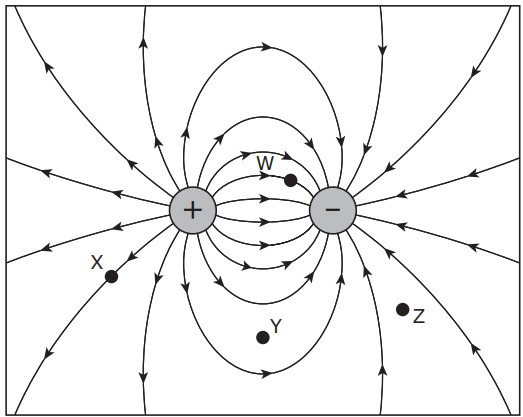
\includegraphics[width=0.4\linewidth]{../figs/PH11-MidSem2-01-5}
\end{center}
\begin{mcq}(4)
	\item W.
	\item X.
	\item Y.
	\item Z.
\end{mcq}
\hideall{
\textbf{Đáp án A.}\\
Tại W các đường sức được vẽ dày hơn các vị trí khác nên cường độ điện trường tai W là lớn nhất so với các vị trí còn lại $\Rightarrow$ lực điện tác dụng lên điện tích đặt tại W là lớn nhất.
}

\item Khi một hạt mang điện bay vào điện trường đều theo phương vuông góc với các đường sức điện thì
\begin{mcq}(2)
	\item tốc độ của hạt giảm dần.
	\item tốc độ của hạt tăng dần.
	\item tốc độ của hạt không đổi.
	\item tốc độ của hạt phụ thuộc vào dấu của điện tích.
\end{mcq}
\hideall{
\textbf{Đáp án B.}\\
Khi điện tích chuyển động trong điện trường đều với vận tốc đầu $\vec{v}_0$ vuông góc với các đường sức điện thì tốc độ của hạt:
$$v=\sqrt{v^2_x+v^2_y}=\sqrt{v^2_0+\left(\dfrac{qE}{m}t\right)^2}.$$
Như vậy, tốc độ của hạt luôn tăng dần.
}

\item Có hai quả cầu kim loại A và B, quả A được cố định trên đế cách điện và quả B được treo bởi sợi dây nhẹ như hình bên dưới. Quả bóng A tích điện âm và được di chuyển từ từ lại gần quả B không tích điện. Mô tả hiện tượng xảy ra.
\begin{center}
	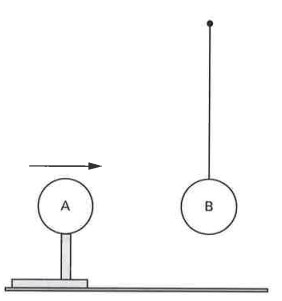
\includegraphics[width=0.35\linewidth]{../figs/PH11-MidSem2-01-6}
\end{center}
\begin{mcq}
	\item Hai quả cầu hút nhau.
	\item Hai quả cầu đẩy nhau.
	\item Ban đầu hai quả cầu hút nhau, sau khi tiếp xúc với nhau thì chúng đẩy nhau.
	\item Ban đầu hai quả cầu đẩy nhau, sau khi tiếp xúc với nhau thì chúng hút nhau.
\end{mcq}
\hideall{
	\textbf{Đáp án C.}\\
	Ban đầu hai quả cầu hút nhau, sau khi tiếp xúc với nhau thì chúng đẩy nhau.
}

\item Bốn điện tích điểm $q_\text{a}$, $q_\text{b}$, $q_\text{c}$, $q_\text{d}$ được cố định tại 4 đỉnh của hình vuông như hình bên. Bốn điện tích có cùng độ lớn. Xác định điều kiện để điện tích $q$ đặt tại tâm của hình vuông cân bằng.
\begin{center}
	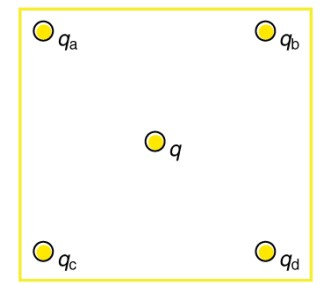
\includegraphics[width=0.4\linewidth]{../figs/PH11-MidSem2-01-7}
\end{center}
\begin{mcq}(2)
	\item $q_\text{a}q_\text{b}>0$ hoặc $q_\text{c}q_\text{d}>0$.
	\item $q_\text{a}q_\text{d}>0$ và $q_\text{b}q_\text{c}>0$.
	\item $q_\text{a}q_\text{b}<0$ hoặc $q_\text{c}q_\text{d}<0$.
	\item $q_\text{a}q_\text{d}<0$ và $q_\text{b}q_\text{c}<0$.
\end{mcq}
\hideall{
	\textbf{Đáp án B.}\\
	$q_\text{a}q_\text{d}>0$ và $q_\text{b}q_\text{c}>0$.
}

\item Cặp điện tích điểm có cùng độ lớn điện tích $q$ đặt trong không khí và cách nhau một khoảng $\ell$ như hình vẽ. Cường độ điện trường do 2 điện tích gây ra tại điểm $P$ có độ lớn và hướng là
\begin{center}
	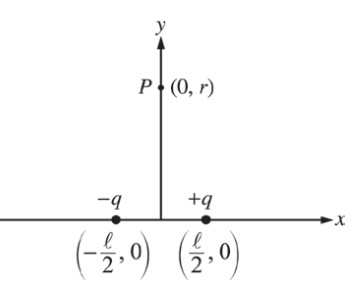
\includegraphics[width=0.4\linewidth]{../figs/PH11-MidSem2-01-2}
\end{center}
\begin{mcq}
	\item $E=\dfrac{1}{4\pi\varepsilon_0}\dfrac{2q}{r^2+\dfrac{\ell^2}{4}}$ và hướng theo chiều $+y$.
	\item $E=\dfrac{1}{4\pi\varepsilon_0}\dfrac{2q}{r^2+\dfrac{\ell^2}{4}}$ và hướng theo chiều $-y$.
	\item $E=\dfrac{1}{4\pi\varepsilon_0}\dfrac{q\ell}{\left(r^2+\dfrac{\ell^2}{4}\right)^{3/2}}$ và hướng theo chiều $-x$.
	\item $E=\dfrac{1}{4\pi\varepsilon_0}\dfrac{q\ell}{\left(r^2+\dfrac{\ell^2}{4}\right)^{3/2}}$ và hướng theo chiều $+x$.
\end{mcq}
\hideall{
\textbf{Đáp án C.}\\
\begin{center}
	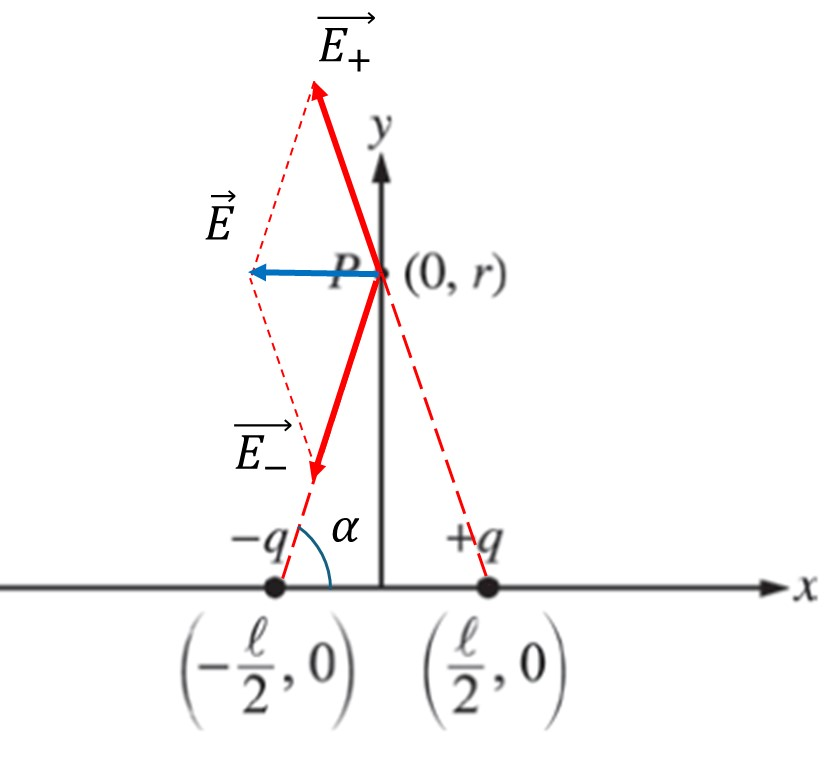
\includegraphics[width=0.4\linewidth]{../figs/PH11-MidSem2-01-3}
\end{center}
Cường độ điện trường tổng hợp tại P:
$$\vec{E}+\vec{E}_++\vec{E}_-$$
Với cường độ điện trường do các điện tích $+q$ và $-q$ gây ra tại P có độ lớn:
$$E_+=E_-=\dfrac{1}{4\pi\varepsilon_0}\dfrac{q}{r^2+\dfrac{\ell^2}{4}}$$
Vì $E_+=E-\Rightarrow \vec{E}//Ox$
$$E=2E_+\cos\alpha=2\cdot\dfrac{1}{4\pi\varepsilon_0}\dfrac{q}{r^2+\dfrac{\ell^2}{4}}\cdot\dfrac{\ell}{2\sqrt{R^2+\dfrac{\ell^2}{4}}}
=\dfrac{1}{4\pi\varepsilon_0}\dfrac{q\ell}{\left(r^2+\dfrac{\ell^2}{4}\right)^{3/2}}.$$}
	\end{enumerate}
\section{Câu trắc nghiệm đúng sai.} 
\textit{Thí sinh trả lời từ câu 1 đến câu 4. Trong mỗi ý \textbf{a)}, \textbf{b)}, \textbf{c)}, \textbf{d)} ở mỗi câu, thí sinh chọn đúng hoặc sai.}
\begin{enumerate}[label=\bfseries Câu \arabic*:]
	\item Hai vật dẫn A và B có kích thước hoàn toàn giống nhau.
	\begin{enumerate}[label=\bfseries \alph*)]
		\item Nếu A và B đặt gần nhau thì hút nhau, điều này chứng tỏ A và B phải nhiễm điện trái dấu.
		\item Có thể làm cho A và B có cùng điện tích bằng cách cho chúng tiếp xúc nhau.
		\item Nếu A và B cùng nhiễm điện, lực tương tác tĩnh điện giữa chúng sẽ càng nhỏ khi chúng cách nhau càng xa.
		\item Nếu A và B nhiễm điện cùng dấu, khi tách A và B ra xa nhau thì lực điện thực hiện công dương.
	\end{enumerate}
\hideall{
\begin{enumerate}[label=\bfseries \alph*)]
	\item Sai. Có thể có trường hợp 1 vật nhiễm điện và 1 vật trung hoà về điện.
	\item Đúng. Hai quả cầu hoàn toàn giống nhau được đặt tiếp xúc với nhau thì chúng sẽ có cùng điện tích.
	\item Đúng. Khoảng cách giữa hai vật nhiễm điện càng lớn thì lực tương tác giữa chúng có độ lớn càng nhỏ.
	\item Đúng. Vì hai vật nhiễm điện cùng dấu nên lực tương tác tĩnh điện giữa hai vật là lực đẩy. Khi tách hai vật xa nhau thì $\vec{F}_\text{đ}\uparrow\uparrow\vec{s}$.
\end{enumerate}
}

\item Nhận định các phát biểu về tụ điện:
\begin{enumerate}[label=\bfseries \alph*)]
	\item Điện dung của tụ điện chỉ phụ thuộc vào kích thước hai bản tụ, không phụ thuộc hình dạng tụ điện.
	\item Điện dung tụ điện phụ thuộc vào chất điện môi giữa hai bản tụ.
	\item Có thể tạo ra bộ tụ có điện dung lớn hơn bằng cách ghép nối tiếp các tụ điện với nhau.
	\item Năng lượng được dự trữ bên trong tụ điện dưới dạng hoá năng của lớp điện môi.
\end{enumerate}
\hideall{
\begin{enumerate}[label=\bfseries \alph*)]
	\item Sai. Điện dung của tụ điện có phụ thuộc vào hình dạng tụ điện.
	\item Đúng. Điện dung tụ điện phụ thuộc vào lớp điện môi giữa hai bản tụ.
	\item Sai. Khi ghép nối tiếp các tụ điện với nhau thì điện dung của bộ tụ sẽ nhỏ hơn điện dung các tụ thành phần.
	\item Sai. Năng lượng được dự trữ bên trong tụ điện dưới dạng năng lượng điện trường.
\end{enumerate}
}

\item Nhận định các phát biểu về đường sức điện:
\begin{enumerate}[label=\bfseries \alph*)]
	\item Vector cường độ điện tại một điểm sẽ tiếp tuyến với đường sức điện tại điểm đó.
	\item Các đường sức điện tạo bởi hệ hai điện tích đặt gần nhau thì có thể cắt nhau nếu hai điện tích trái dấu.
	\item Đường sức điện luôn là đường thẳng.
	\item Cường độ điện trường tại một vị trí bất kì càng lớn nếu đường sức nơi đó càng dày.
\end{enumerate}
\hideall{
\begin{enumerate}[label=\bfseries \alph*)]
	\item Đúng.
	\item Sai. Các đường sức điện không cắt nhau.
	\item Sai. Các đường sức điện không phải bao giờ cũng là đường thẳng.
	\item Đúng.
\end{enumerate}
}

\item Một electron được bắn vào vùng không gian giữa hai bản phẳng tích điện trái dấu theo phương song song với mặt phẳng hai bản với động năng ban đầu $W_\text{đ}=\SI{1.1375}{\milli\electronvolt}$. Chiều dài mỗi bản là $\SI{10}{\centi\meter}$. Hai bản được đặt cách nhau $\SI{10}{\centi\meter}$ và hiệu điện thế giữa hai bản là $\SI{75}{\volt}$. Bỏ qua tác dụng của trọng lực, khối lượng của electron $m_e=\SI{9.1E-31}{\kilogram}$. Ban đầu electron ở sát bản âm.
\begin{enumerate}[label=\bfseries \alph*)]
	\item Electron chuyển động nhanh dần đều.
	\item Tốc độ ban đầu của electron là $\SI{2E4}{\meter/\second}$.
	\item Cường độ điện trường giữa hai bản là $\SI{750}{\volt/\centi\meter}$.
	\item Electron sẽ chạm vào bản tích điện dương.
\end{enumerate}
\hideall{
\begin{enumerate}[label=\bfseries \alph*)]
	\item Sai. Electron chuyển động như vật ném ngang với vận tốc phụ thuộc theo thời gian $v=\sqrt{v^2_0+\left(\dfrac{\left|e\right|Ut}{m_ed}\right)^2}$.
	\item Đúng. $v_0=\sqrt{\dfrac{2W_\text{đ}}{m_e}}=\SI{2E4}{\meter/\second}$.
	\item Sai. Cường độ điện trường giữa hai bản $E=\dfrac{U}{d}=\SI{7.5}{\volt/\centi\meter}$.
	\item Đúng. \\
	Thời gian cần thiết để electron rời khỏi hai bản:
	$$t_1=\dfrac{\ell}{v_0}=\SI{5E-6}{\second}.$$
	Thời gian để electron có thể chạm vào bản dương:
	$$t_2=\sqrt{\dfrac{2d}{\dfrac{\left|e\right|U}{m_ed}}}\approx\SI{3.9E-8}{\second}.$$
	Vì $t_2<t_1$ nên electron sẽ chạm vào bản dương trước khi có thể rời khỏi vùng không gian giữa hai bản.
\end{enumerate}
}
\end{enumerate}
\section{Câu trắc nghiệm trả lời ngắn.} \textit{Thí sinh trả lời từ câu 1 đến câu 6.}
\begin{enumerate}[label=\bfseries Câu \arabic*:]
	\item M và N là hai điểm trong điện trường có điện thế $V_\text{M}=\SI{25}{\volt}$ và $V_\text{N}=\SI{40}{\volt}$. Hiệu điện thế giữa hai điểm M và N là bao nhiêu volt?
	\hideall{
		Hiệu điện thế giữa hai điểm M và N:
		$$U_\text{MN}=V_\text{M}-V_\text{N}=\SI{-15}{\volt}.$$
	}
	
	\item Có ba cặp điện tích điểm như hình vẽ. Mỗi cặp điện tích được đặt cách nhau một khoảng $d$ nhất định. Sắp xếp độ lớn lực tương tác tĩnh điện giữa mỗi cặp điện tích theo thứ tự tăng dần.
	\begin{center}
		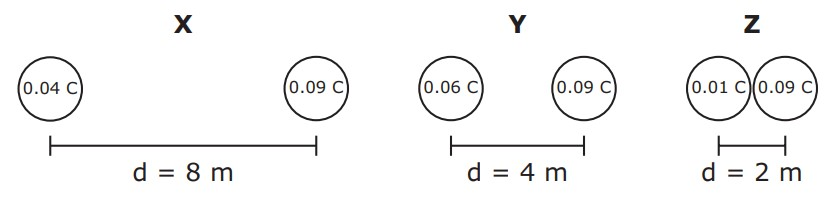
\includegraphics[width=0.8\linewidth]{../figs/PH11-MidSem2-01-4}
	\end{center}
\hideall{
$$X\rightarrow Z\rightarrow Y.$$
}



\item Hai điện tích $q_1=4q$ và $q_2=-q$ đặt tại hai điểm A và B cách nhau $\SI{9}{\centi\meter}$ trong chân không. Vị trí có cường độ điện trường tổng hợp bằng 0 cách B một khoảng bao nhiêu \textit{(tính theo centimet)}?
\hideall{
$\SI{9}{\centi\meter}.$
}

\item Bộ tụ điện trong đèn chụp ảnh có điện dung $\SI{750}{\micro\farad}$ được tích điện đến hiệu điện thế $\SI{330}{\volt}$. Mỗi lần đèn loé sáng, tụ điện phóng điện trong thời gian $\SI{5}{\milli\second}$. Tính công suất phóng điện của tụ \textit{(làm tròn đến 2 chữ số thập phân)} là bao nhiêu $\si{\kilo\watt}$.
\hideall{
$\SI{8.17}{\kilo\watt}.$
}

\item Hai tụ điện có điện dung $C_1=\SI{12.8}{\micro\farad}$, $C_2=\SI{32}{\micro\farad}$ được mắc thành bộ tụ nối tiếp, sau đó được nối vào hiệu điện thế $U=\SI{63}{\volt}$. Tính hiệu điện thế giữa hai đầu tụ $C_1$ theo đơn vị volt.
\hideall{
$\SI{45}{\volt}.$
}

\item Trong không khí có ba điểm thẳng hàng theo đúng thứ tự O, M, A sao cho $\text{OM}=\text{OA}/3$. Khi đặt tại O điện tích điểm $9Q$ thì độ lớn cường độ điện trường tại A là $\SI{900}{\volt/\meter}$. Khi đặt tại O điện tích điểm $7Q$ thì độ lớn cường độ điện trường tại M là bao nhiêu \textit{(tính theo đơn vị $\si{\volt/\meter}$)}?
\hideall{
	$$\dfrac{E_\text{M}}{E_\text{A}}=\dfrac{\dfrac{k\left|7Q\right|}{OM^2}}{\dfrac{k\left|9Q\right|}{OA^2}}=\dfrac{7}{9}\left(\dfrac{OA}{OM}\right)^2=7\Rightarrow E_\text{M}=\SI{6300}{\volt/\meter}.$$
}
\begin{center}
	\textbf{--- HẾT ---}
\end{center}


\end{enumerate}